% Options for packages loaded elsewhere
\PassOptionsToPackage{unicode}{hyperref}
\PassOptionsToPackage{hyphens}{url}
\PassOptionsToPackage{dvipsnames,svgnames,x11names}{xcolor}
%
\documentclass[
  letterpaper,
  DIV=11,
  numbers=noendperiod]{scrartcl}

\usepackage{amsmath,amssymb}
\usepackage{iftex}
\ifPDFTeX
  \usepackage[T1]{fontenc}
  \usepackage[utf8]{inputenc}
  \usepackage{textcomp} % provide euro and other symbols
\else % if luatex or xetex
  \usepackage{unicode-math}
  \defaultfontfeatures{Scale=MatchLowercase}
  \defaultfontfeatures[\rmfamily]{Ligatures=TeX,Scale=1}
\fi
\usepackage{lmodern}
\ifPDFTeX\else  
    % xetex/luatex font selection
\fi
% Use upquote if available, for straight quotes in verbatim environments
\IfFileExists{upquote.sty}{\usepackage{upquote}}{}
\IfFileExists{microtype.sty}{% use microtype if available
  \usepackage[]{microtype}
  \UseMicrotypeSet[protrusion]{basicmath} % disable protrusion for tt fonts
}{}
\makeatletter
\@ifundefined{KOMAClassName}{% if non-KOMA class
  \IfFileExists{parskip.sty}{%
    \usepackage{parskip}
  }{% else
    \setlength{\parindent}{0pt}
    \setlength{\parskip}{6pt plus 2pt minus 1pt}}
}{% if KOMA class
  \KOMAoptions{parskip=half}}
\makeatother
\usepackage{xcolor}
\setlength{\emergencystretch}{3em} % prevent overfull lines
\setcounter{secnumdepth}{-\maxdimen} % remove section numbering
% Make \paragraph and \subparagraph free-standing
\makeatletter
\ifx\paragraph\undefined\else
  \let\oldparagraph\paragraph
  \renewcommand{\paragraph}{
    \@ifstar
      \xxxParagraphStar
      \xxxParagraphNoStar
  }
  \newcommand{\xxxParagraphStar}[1]{\oldparagraph*{#1}\mbox{}}
  \newcommand{\xxxParagraphNoStar}[1]{\oldparagraph{#1}\mbox{}}
\fi
\ifx\subparagraph\undefined\else
  \let\oldsubparagraph\subparagraph
  \renewcommand{\subparagraph}{
    \@ifstar
      \xxxSubParagraphStar
      \xxxSubParagraphNoStar
  }
  \newcommand{\xxxSubParagraphStar}[1]{\oldsubparagraph*{#1}\mbox{}}
  \newcommand{\xxxSubParagraphNoStar}[1]{\oldsubparagraph{#1}\mbox{}}
\fi
\makeatother


\providecommand{\tightlist}{%
  \setlength{\itemsep}{0pt}\setlength{\parskip}{0pt}}\usepackage{longtable,booktabs,array}
\usepackage{calc} % for calculating minipage widths
% Correct order of tables after \paragraph or \subparagraph
\usepackage{etoolbox}
\makeatletter
\patchcmd\longtable{\par}{\if@noskipsec\mbox{}\fi\par}{}{}
\makeatother
% Allow footnotes in longtable head/foot
\IfFileExists{footnotehyper.sty}{\usepackage{footnotehyper}}{\usepackage{footnote}}
\makesavenoteenv{longtable}
\usepackage{graphicx}
\makeatletter
\def\maxwidth{\ifdim\Gin@nat@width>\linewidth\linewidth\else\Gin@nat@width\fi}
\def\maxheight{\ifdim\Gin@nat@height>\textheight\textheight\else\Gin@nat@height\fi}
\makeatother
% Scale images if necessary, so that they will not overflow the page
% margins by default, and it is still possible to overwrite the defaults
% using explicit options in \includegraphics[width, height, ...]{}
\setkeys{Gin}{width=\maxwidth,height=\maxheight,keepaspectratio}
% Set default figure placement to htbp
\makeatletter
\def\fps@figure{htbp}
\makeatother

% load packages
\usepackage{geometry}
\usepackage{xcolor}
\usepackage{eso-pic}
\usepackage{fancyhdr}
\usepackage{sectsty}
\usepackage{fontspec}
\usepackage{titlesec}
\usepackage{atbegshi} % Add this package

%% Set page size with a wider right margin
\geometry{a4paper, total={170mm,257mm}, left=10mm, top=10mm, bottom=5mm, right=10mm}

%% Let's define some colours
\definecolor{light}{HTML}{E6E6FA}
\definecolor{highlight}{HTML}{800080}
\definecolor{dark}{HTML}{f44336}

%% Let's add the border on the right hand side 
\AddToShipoutPictureBG*{% 
    \AtPageLowerLeft{% 
        \put(\LenToUnit{\dimexpr\paperwidth-0cm},0){% 
            \color{light}\rule{0cm}{\LenToUnit\paperheight}%
          }%
     }%
}

%% Add the logo only on the first page
\AddToShipoutPictureBG*{\AtTextLowerLeft{% 
    \ifnum\value{page}=1
        \put(\LenToUnit{\dimexpr\paperwidth-3.25cm},26.2cm){% move it to the top right
            \color{light}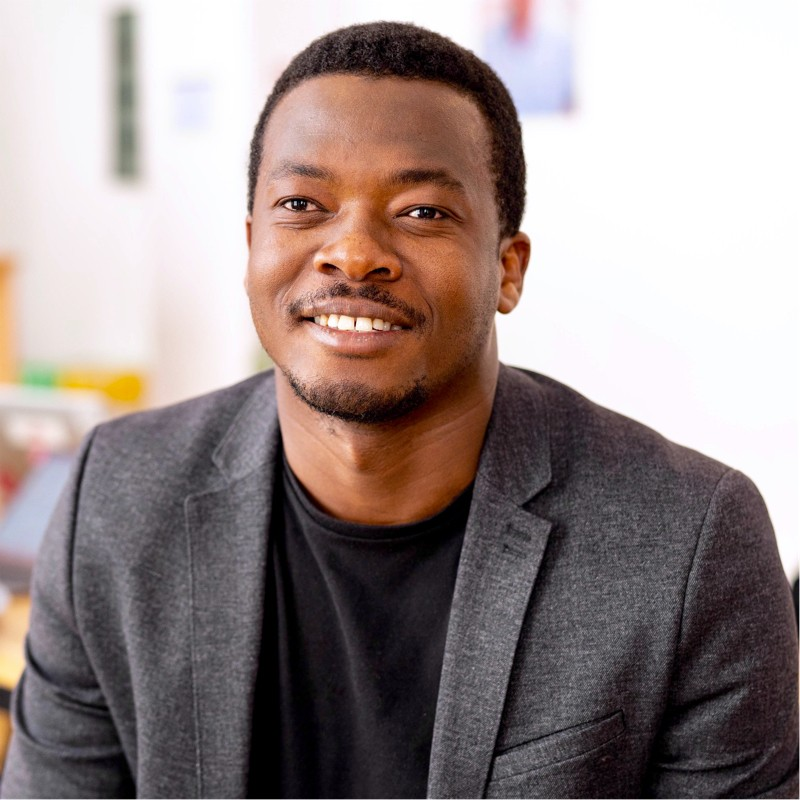
\includegraphics[width=1.5cm]{_extensions/nrennie/PrettyPDF/logo.png}
          }%
    \fi
}}

%% Style the page number
\fancypagestyle{mystyle}{
  \fancyhf{}
  \renewcommand\headrulewidth{0pt}
  \fancyfoot[R]{\thepage}
  \fancyfootoffset{3.5cm}
}

\setlength{\footskip}{20pt}

%% style the chapter/section fonts
\chapterfont{\color{dark}\fontsize{20}{16.8}\selectfont}
\sectionfont{\color{blue}\fontsize{20}{10}\selectfont}
\subsectionfont{\color{red}\fontsize{8}{10}\selectfont}
\titleformat{\subsection}
  {\color{blue}\sffamily\Large\bfseries}{\thesubsection}{1em}{}[{\titlerule[0.8pt]}]
\titlespacing*{\subsection}{0pt}{*0}{*0}

%% Reduce space before and after section titles
\titlespacing*{\section}{0pt}{*0}{*0}

% left align title
\makeatletter
\renewcommand{\maketitle}{\bgroup\setlength{\parindent}{0pt}
\begin{flushleft}
  {\sffamily\huge\textbf{\MakeUppercase{\@title}}} \vspace{0.01cm} \newline
  {\Large {\@subtitle}}
  \@author
\end{flushleft}\egroup
}
\makeatother

%% Use some custom fonts
\setsansfont{Ubuntu}[
    Path=_extensions/nrennie/PrettyPDF/Ubuntu/,
    Scale=0.9,
    Extension = .ttf,
    UprightFont=*-Regular,
    BoldFont=*-Bold,
    ItalicFont=*-Italic,
    ]

\setmainfont{Ubuntu}[
    Path=_extensions/nrennie/PrettyPDF/Ubuntu/,
    Scale=0.9,
    Extension = .ttf,
    UprightFont=*-Regular,
    BoldFont=*-Bold,
    ItalicFont=*-Italic,
    ]
\KOMAoption{captions}{tableheading}
\makeatletter
\@ifpackageloaded{caption}{}{\usepackage{caption}}
\AtBeginDocument{%
\ifdefined\contentsname
  \renewcommand*\contentsname{Table of contents}
\else
  \newcommand\contentsname{Table of contents}
\fi
\ifdefined\listfigurename
  \renewcommand*\listfigurename{List of Figures}
\else
  \newcommand\listfigurename{List of Figures}
\fi
\ifdefined\listtablename
  \renewcommand*\listtablename{List of Tables}
\else
  \newcommand\listtablename{List of Tables}
\fi
\ifdefined\figurename
  \renewcommand*\figurename{Figure}
\else
  \newcommand\figurename{Figure}
\fi
\ifdefined\tablename
  \renewcommand*\tablename{Table}
\else
  \newcommand\tablename{Table}
\fi
}
\@ifpackageloaded{float}{}{\usepackage{float}}
\floatstyle{ruled}
\@ifundefined{c@chapter}{\newfloat{codelisting}{h}{lop}}{\newfloat{codelisting}{h}{lop}[chapter]}
\floatname{codelisting}{Listing}
\newcommand*\listoflistings{\listof{codelisting}{List of Listings}}
\makeatother
\makeatletter
\makeatother
\makeatletter
\@ifpackageloaded{caption}{}{\usepackage{caption}}
\@ifpackageloaded{subcaption}{}{\usepackage{subcaption}}
\makeatother
\makeatletter
\@ifpackageloaded{tcolorbox}{}{\usepackage[skins,breakable]{tcolorbox}}
\makeatother
\makeatletter
\@ifundefined{shadecolor}{\definecolor{shadecolor}{rgb}{.97, .97, .97}}{}
\makeatother
\makeatletter
\@ifundefined{codebgcolor}{\definecolor{codebgcolor}{named}{light}}{}
\makeatother
\makeatletter
\ifdefined\Shaded\renewenvironment{Shaded}{\begin{tcolorbox}[frame hidden, breakable, sharp corners, enhanced, colback={codebgcolor}, boxrule=0pt]}{\end{tcolorbox}}\fi
\makeatother

\ifLuaTeX
  \usepackage{selnolig}  % disable illegal ligatures
\fi
\usepackage{bookmark}

\IfFileExists{xurl.sty}{\usepackage{xurl}}{} % add URL line breaks if available
\urlstyle{same} % disable monospaced font for URLs
\hypersetup{
  colorlinks=true,
  linkcolor={highlight},
  filecolor={Maroon},
  citecolor={Blue},
  urlcolor={highlight},
  pdfcreator={LaTeX via pandoc}}


\author{}
\date{}

\begin{document}

\pagestyle{mystyle}


\section{Lewis Hounkpevi \textbar{} Senior Data Scientist \textbar{} ML
Engineer}\label{lewis-hounkpevi-senior-data-scientist-ml-engineer}

\begin{center}Forte expertise en AI/ML, Python, R, AWS Cloud\end{center}

\textbf{Ville :} xxxxxxxxxx \textbar{} \textbf{Tél :} +33 x xx xx xx
xx~\textbar{} \textbf{Email :}
\href{mailto:dumesnil.hounkpevi@gmail.com}{\nolinkurl{dumesnil.hounkpevi@gmail.com}}~\\
\textbf{LinkedIn :} \url{https://www.linkedin.com/in/lewishounkpevi}
\textbar{} \textbf{Github :} \url{https://github.com/lewishounkpevi}

\subsection{Compétences}\label{compuxe9tences}

\begin{itemize}
\tightlist
\item
  \textbf{Environnement Technique :} Expert en R et Python, SQL, Git,
  Gitlab, AWS Sagemaker, S3, Redshift, Docker, PowerBI
\item
  \textbf{Machine Learning et MLOps:}

  \begin{itemize}
  \tightlist
  \item
    Pipeline : Xgboost, GBM, Random Forest, KMeans, CAH, Dbscan, Deep
    Learning
  \item
    Mise en production et Monitoring : MLflow, FastApi, Flask, CI/CD,
    AWS SageMaker, AWS CodeBuild
  \end{itemize}
\item
  \textbf{Analyse de données :} Détection anomalies, modélisation et
  scoring, segmentation, évaluation de risques ou d'appétence
\item
  \textbf{Soft skills :} Mise en place de la stratégie Data, Leadership,
  Communication, Pédagogie
\item
  \textbf{Langues :} Anglais : Courant
\end{itemize}

\subsection{Expérience
Professionnelle}\label{expuxe9rience-professionnelle}

\emph{Juil 2022 -- En cours} : \textbf{Senior Data Scientist -- Santevet
-- Full remote}

Ma mission est de conduire toutes les études et analyses relatives au
churn et d'aider les différents corps de métier (Actuariat, Finance,
Marketing et Commerce) dans leur contribution à réduite le churn tout en
étant Lead technique d'une équipe de 3 collaborateurs.

\textbf{Réalisations Clés :}

\begin{itemize}
\tightlist
\item
  Réduction du churn de 10\% en utilisant des modèles de scoring.
\item
  Mise en production et monitoring de 5 modèles de prédiction sous
  Python et AWS SageMaker, S3 et Redshift
\item
  Segmentations et profilages du portefeuille client ayant conduit à la
  mise en place de plans d'actions de rétention et de fidélisation des
  clients
\item
  Amélioration de l'efficacité de l'équipe de 20\% en automatisant les
  processus d'analyse.
\end{itemize}

\emph{Sept 2019 -- Juin 2022} : \textbf{Senior Data Scientist à la
Direction des Etudes et Analyses -- Unédic -- Paris}

Mission principale : Accompagnement technique et montée en compétence de
l'équipe de l'Unédic sur les nouveaux outils d'analyse de données, en
apportant mon expertise dans les études et travaux d'analyse.

\textbf{Réalisations Clés :}

\begin{itemize}
\tightlist
\item
  Publication de 5 articles techniques sur l'analyse des demandeurs
  d'emploi.
\item
  Formation de plus de 10 collaborateurs sur les outils modernes de data
  science R, Python, Spark et Git.
\end{itemize}

\emph{Fév 2018 -- Août 2019} : \textbf{Lead Data Scientist à la
Direction Marketing -- Eni Gas \& Power -- Levallois}

Mission principale : Responsable de l'analyse statistique, modélisation
et suivi des KPI pour les segments B2C et B2B

\textbf{Réalisations Clés :}

\begin{itemize}
\tightlist
\item
  Mise en production de scores de churn, de cross-sell et d'appétence
  aux services pour les offres, contribuant à réduire le churn de 10\%
  et augmenter le cross-sell de 15\%.
\item
  Détection des différents profils des clients en portefeuille.
\item
  Développement de 3 packages R augmentant la productivité de 25\%.
\end{itemize}

\emph{Mai 2014 -- Jan 2018} : \textbf{Responsable technique Data
Scientist - Consulting pour Renault (Altran, Ligeron) -- Paris}

\begin{itemize}
\tightlist
\item
  4 ans d'expérience en data science, avec une expertise en ML,
  utilisant R, Python et SQL, Git.
\item
  Compétences en automatisation de rapports d'analyse et en
  visualisation de données avec un souci de clarté, pédagogie et
  précision dans l'analyse de données.
\end{itemize}

\subsection{Formation}\label{formation}

\begin{itemize}
\tightlist
\item
  \textbf{Specialization in Building Cloud Computing Solutions at Scale}
  - Duke University - USA (Coursera) - 2024
\item
  \textbf{Master 2 en Ingénierie Statistique} - Université de
  Cergy-Pontoise - France - 2014
\end{itemize}




\end{document}
